
\documentclass{esub2acm}
%\documentclass[11pt]{article}

\usepackage{alltt}
\usepackage{graphicx}
%\usepackage[dvips]{epsfig}
% New mathematical facilities like \mathbb, \big, and \mapsto
%\usepackage{amssymb}
% Defines page size and margins.
%%
%   Preamble
%
%
%   The parameter oddsidemargin (evensidemargin) is one inch 
%   less than the distance from the edge of the paper to the 
%   left margin of the text on right-hand (left-hand) pages. 
%
\setlength{\textwidth}{6.0in}
\setlength{\oddsidemargin}{23pt}
\setlength{\evensidemargin}{23pt}
\setlength{\topmargin}{-0.5in}
\setlength{\textheight}{8.5in}

%   Some abbreviations

\newcommand{\grad}{\nabla}
\newcommand{\bull}{\vrule height 1.8ex width 1.0ex depth 0ex}
\newcommand{\half}{{\textstyle{\frac{1}{2}}}}
\newcommand{\Ref}[1]{\mbox{\rm{(\ref{#1})}}}
\newcommand{\qed}{$ \blacksquare $ \medskip}
\newcommand{\lt}{<}
\newcommand{\gt}{>}
%
%   Enviroments theorem lemma and algorithm are created, and all
%   three are numbered as in theorem.
%
\newtheorem{theorem}{Theorem}
\newtheorem{lemma}[theorem]{Lemma}
\newtheorem{corollary}[theorem]{Corollary}
\newtheorem{algorithm}[theorem]{Algorithm}
\newtheorem{definition}[theorem]{Definition}
\newtheorem{assumption}[theorem]{Assumption}
%
%   The numbering below can be done with the numinsec style
%   provided by SIAM.
%
%   The theorem numbers are defined to be of the form section#.theorem#
%
\renewcommand{\thetheorem}{\thesection.\arabic{theorem}}
%
%   Defines the equation number to be of the form section#.equation#
%
%   \renewcommand{\theequation}{\thesection.\arabic{equation}}
%
%   Defines the figure and table numbers to be of the form 
%   section#.figure# and section#.table#
%
\renewcommand{\thefigure}{\thesection.\arabic{figure}}
\renewcommand{\thetable}{\thesection.\arabic{table}}


% Redefines the size of the section headings.
%\usepackage{../sty/art11mod}
% The float package is described in page 146 of the LaTeX companion.
\usepackage{../sty/float}
% Numbers equations,... consecutively within sections.
%\usepackage{../sty/numinsec}
% The bar package is described in page 283 of the LaTeX companion.
%\usepackage{../sty/bar}
% The url package is intended for email addresses, hypertext links, ...
\usepackage{../sty/url}

%\usepackage[first]{draftcopy}
%\usepackage{subfigure}

% New commands for final copy
\newcommand{\Ref}{\ref}
\newcommand{\half}{\frac{1}{2}}
\newcommand{\lt}{<}
\newcommand{\gt}{>}
\newcommand{\grad}{\nabla}

% New commands
%\newcommand{\R}{\mbox{${\mathbb R}$}}
\newcommand{\R}{\mbox{${\Re}$}}
\newcommand{\Note}{\marginpar[$\Rightarrow$]{$\Leftarrow$}}
% Renewing commands
\renewcommand{\thefootnote}{\fnsymbol{footnote}}
% Algorithm floating environment.
\newfloat{Algorithm}{thp}{loa}[section]

% Calligraphic letter abbreviations.

\newcommand{\cA} {\mbox{$\cal A$}}
\newcommand{\cB} {\mbox{$\cal B$}}
\newcommand{\cD} {\mbox{$\cal D$}}
\newcommand{\cF} {\mbox{$\cal F$}}
\newcommand{\cI} {\mbox{$\cal I$}}

\begin{document}
%\setlength{\baselineskip}{15pt}

%\pagestyle {empty}

%  
\vspace{1.75in}

\begin{center}

ARGONNE NATIONAL LABORATORY

9700 South Cass Avenue

Argonne, Illinois  60439

\vspace{1.5in}

{\Large
{\bf 
TAO 3.9 Users Manual
}
}

\vspace{.5in}

{\bf Alp Dener \\ Todd Munson \\ Jason Sarich \\ Stefan Wild \\ Steven Benson \\ Lois Curfman McInnes}

\vspace{.5in}

Mathematics and Computer Science Division

\vspace{.25in}

Technical Memorandum ANL/MCS-TM-322

\vspace{.25in}

This manual is intended for use with TAO version 3.9

\vspace{1.0in}

\today
\end{center}

\vspace{0.75in}

\par\noindent
This product includes software produced by UChicago Argonne, LLC under 
Contract No. DE-AC02-06CH11357 with the Department of Energy.

%  \newpage
%  \mbox{}
%  \newpage

%\pagestyle{plain}


\title{A Case Study in the Performance and Scalability of
Optimization Algorithms\footnotemark}

\author{Steven J. Benson
\and
Lois Curfman McInnes
\and
Jorge J. Mor\'e \\
Mathematics and Computer Science Division \\
Argonne National Laboratory
}

\begin{abstract}
We analyze the performance and scalabilty of algorithms for the
solution of large optimization problems on 
high-performance parallel architectures.
Our case study uses the GPCG (gradient projection, conjugate gradient) algorithm
for solving bound-constrained convex quadratic problems.
Our implementation of the GPCG algorithm within the Toolkit for 
Advanced Optimization (TAO) is available
for a wide range of high-performance architectures
and has been tested on problems with over 2.5 million variables.
We analyze the performance as a function of the number of variables, 
the number of
free variables, and the preconditioner.
In addition, we discuss how the software
design facilitates algorithmic comparisons.
\end{abstract}

%  \noindent
%  {\bf Key words.} 
%  large-scale optimization,
%  high-performance architectures,
%  conjugate gradients, 
%  gradient projection,
%  quadratic programming., 

\category{G.4.m} {Mathematical Software} {Parallel and vector implementations}
\category{D.2.13} {Reusable Software} {Reusable libraries}
\category{G.1.6}{Optimization}{Quadratic Programming Methods}
\terms{Bound constrained optimization, Parallel Efficiency}
\keywords{}
\begin{bottomstuff}
This work was supported by the Mathematical, Information, and
Computational Sciences Division subprogram of the Office of Advanced
Scientific Computing, U.S. Department of Energy, under Contract
W-31-109-Eng-38.
\begin{authinfo}
\end{authinfo}
\permission
\end{bottomstuff}
\markboth{S.J. Benson, L. McInnes, J.J. Mor\'e}
     {A Case Study in the Performance and Scalability of
Optimization Algorithms}
\maketitle


%
%  Introduction to PETSc
%
%
% Note that we use a modified version of report.sty, so that tables and
% figures are numbered consecutively throughout the document (not by
% chapters).  
%
\documentclass[twoside,12pt]{../sty/report_petsc}

\usepackage{makeidx,xspace}
\usepackage[bookmarksopen,colorlinks]{hyperref}
\usepackage{color}
\input pdfcolor.tex     

\usepackage[pdftex]{graphicx}

%\usepackage{psfig}
\usepackage{../sty/verbatim}
\usepackage{../sty/tpage}
\usepackage{../sty/here}
\usepackage{../sty/anlhelper}
\usepackage{../sty/trl}

\setlength{\textwidth}{6.5in}
\setlength{\oddsidemargin}{0.0in}
\setlength{\evensidemargin}{0.0in}
\setlength{\textheight}{9.2in}
\setlength{\topmargin}{-.8in}

\newcommand{\findex}[1]{\index{FUNCTION #1}}
\newcommand{\sindex}[1]{\index{#1}}
 
% Defines the environment where design issues are discussed. In the manual
% version of this report, these regions are ignored.
\def\design{\medskip \noindent Design Issue:\begin{em}}
\def\enddesign{\end{em} \medskip}
% Manual version:
% \def\design{\comment}
% \def\enddesign{\endcomment}

% Print DRAFT in large letters across every page
% \special{!userdict begin /bop-hook{gsave 200 70 translate
% 65 rotate /Times-Roman findfont 216 scalefont setfont
% 0 0 moveto 0.95 setgray (DRAFT) show grestore}def end}

% Defines that we're doing the short intro part, not the whole manual,
% used in part1.tex.
\def\shortintro{*}
\renewcommand{\cite}[1]{}
\def\thesection {$\!\!\!\!$}

\begin{document}

\begin{center}
$\!$
\vspace{1.0cm}
\thispagestyle{empty}

{\huge \bf Introduction to PETSc}\\ 
\vspace{0.5cm}
{\LARGE (Part I of the PETSc Users Manual)} \\
\vspace{1.5cm}
{\large \em Satish Balay\\Kris Buschelman\\Victor Eijkhout\\William Gropp\\Dinesh Kaushik\\Matt Knepley\\Lois Curfman McInnes\\Barry Smith\\Hong Zhang\\
\medskip \medskip
Mathematics and Computer Science Division\\
Argonne National Laboratory\\
9700 South Cass Avenue\\
Argonne, IL 60439-4844\\
\medskip
 2008}
\end{center}

\vspace{1.0cm}

% Abstract for TAO Users Manual

\addcontentsline{toc}{chapter}{Preface}
\section*{Preface}

The Toolkit for Advanced Optimization (TAO) focuses on the development
of algorithms and software for the solution of large-scale optimization 
problems on high-performance architectures.  Areas of interest include 
unconstrained and bound-constrained optimization, nonlinear least squares 
problems, optimization problems with partial differential equation 
constraints, and variational inequalities and complementarity 
constraints.

The development of TAO was motivated by the scattered support for
parallel computations and the lack of reuse of external toolkits in
current optimization software.  Our aim is to produce high-quality 
optimization software for computing environments ranging from 
workstations and laptops to massively parallel high-performance 
architectures.  Our design decisions are strongly motivated by 
the challenges inherent in the use of large-scale distributed 
memory architectures and the reality of working with large, 
often poorly structured legacy codes for specific 
applications.

This manual describes the use of TAO 2.2.0.  Since TAO is still under 
development, changes in usage and calling sequences may occur.  TAO 
is fully supported; see the the web site \url{http://www.mcs.anl.gov/tao} 
for information on contacting the developers.

%%% Local Variables: 
%%% mode: latex
%%% TeX-master: "manual_tex"
%%% End: 



\noindent {\bf Note:} This document serves as the first section of the {\em PETSc Users
Manual}, which elaborates on the use and design of PETSc. The
manual and is available in its entirety via the World Wide Web at
the PETSc home page, {\tt http://www.mcs.anl.gov/petsc}.
When referencing PETSc, please do 
not refer to this document. Instead reference the following: Satish
Balay, Kris Buschelman, Victor Eijhout, William Gropp, Dinesh Kaushik, 
Lois Curfman McInnes, Barry Smith and Hong Zhang.  {\em
PETSc Users Manual}, Technical Report ANL-95/11 - Revision 3.0.0,
Argonne National Laboratory, 2008.

%
% Acknowledgements for users manual
\newpage
% Acknowledgements for PETSc Users Manual
%
% These are also listed on the PETSc homepage, so if you add something here
% add it to the home page also
%
\noindent {\bf Acknowledgments:}

\medskip \medskip \noindent
We thank all PETSc users for their many suggestions, bug reports, and
encouragement.  We especially thank Victor Eijkhout, David Keyes, and
Matthew Knepley for their valuable comments on the source code,
functionality, and documentation for PETSc.


\vspace{.3in}
\noindent
Some of the source code and utilities in PETSc (or software used by PETSc)
have been written by 
\begin{itemize}
  \item Mark Adams, scalability features of MPIBAIJ matrices,
  \item Allison Baker, the flexible GMRES code,
  \item Tony Caola, the SPARSEKIT2 ilutp() interface,
  \item Chad Carroll, Win32 graphics,
  \item Cameron Cooper, portions of the VecScatter routines, 
  \item Victor Eijkhout, KSP type BICG, VecPipeline() and VecXXXBegin()/End() routines, 
  \item Paulo Goldfeld, balancing Neumann-Neumann preconditioner,
  \item Matt Hille, 
  \item Matthew Knepley,
  \item Domenico Lahaye, the interface to John Ruge and Klaus Stueben's AMG,
  \item Peter Mell, portions of the DA routines,
  \item Todd Munson, the LUSOL (sparse solver in MINOS) interface,
  \item Wing-Lok Wan, the ILU portion of BlockSolve95,
  \item Liyang Xu, the interface to PVODE.
\end{itemize}

\vspace{.3in}
\noindent
PETSc uses routines from 
\begin{itemize}
  \item BLAS
  \item LAPACK
  \item LINPACK      matrix factorization and solve; converted to C using {\tt f2c} and then 
                      hand-optimized for small matrix sizes, for block matrix data structures,
  \item MINPACK      sequential matrix coloring routines for finite difference Jacobian
                       evaluations; converted to C using {\tt f2c},
  \item SPARSPAK     matrix reordering routines, converted to C using {\tt f2c},
  \item SPARSEKIT2   written by Yousef Saad, iludtp(), converted to C using {\tt f2c}. These routines 
                     are copyrighted by Saad under the GNU copyright, see \trl{${PETSC_DIR}/src/mat/impls/aij/seq/ilut.c}.
  \item libtfs the efficient, parallel direct solver developed by Henry Tufo and Paul Fischer.
\end{itemize}


\vspace{.3in}
\noindent
PETSc interfaces to the following external software:
\begin{itemize}
  \item AMG          the algebraic multigrid code of John Ruge and Klaus Stueben,
                     \trllink{http://www.mgnet.org/mgnet-codes-gmd.html}{http://www.mgnet.org/mgnet-codes-gmd.html}
  \item BlockSolve95 for parallel ICC(0) and ILU(0) preconditioning,
                     \trllink{http://www.mcs.anl.gov/blocksolve}{http://www.mcs.anl.gov/blocksolve},
  \item ESSL         IBM's math library for fast sparse direct LU factorization,
  \item LUSOL        sparse LU factorization code (part of MINOS) developed by Michael Saunders,
                      Systems Optimization Laboratory, Stanford University,
                     \trllink{http://www.sbsi-sol-optimize.com/}{http://www.sbsi-sol-optimize.com/},
  \item Matlab       
  \item ParMeTiS      parallel graph partitioner, \trllink{http://www-users.cs.umn.edu/~karypis/metis/}{http://www-users.cs.umn.edu/~karypis/metis/},
  \item PVODE        parallel ODE integrator, \trllink{http://www.llnl.gov/CASC/PVODE}{http://www.llnl.gov/CASC/PVODE},
  \item SPAI         for parallel sparse approximate inverse preconditiong, 
                     \trllink{http://www.sam.math.ethz.ch/~grote/spai/}{http://www.sam.math.ethz.ch/~grote/spai/}.
\end{itemize}
These are all optional packages and do not need to be installed to use PETSc.




\newpage
% Include only Part 1 of users manual 
\section{Introduction}
% $Id: part1.tex,v 1.146 2001/08/22 18:03:15 balay Exp $ 

% --------------------------------------------------------------------
%
%                            PART 1
%
%   This introductory PETSc information is included in 
%   both manual.tex and intro.tex.
%
% --------------------------------------------------------------------

\label{sec_gettingstarted}

The Portable, Extensible Toolkit for Scientific Computation (PETSc)
has successfully demonstrated that the use of modern programming
paradigms can ease the development of large-scale scientific
application codes in Fortran, C, and C++.  Begun several years ago,
the software has evolved into a powerful set of tools for the
numerical solution of partial differential equations and related problems 
on high-performance computers.

PETSc consists of a variety of libraries (similar to classes in C++),
which are discussed in detail in Parts II and III of the users manual.
Each library manipulates a particular family of objects (for instance,
vectors) and the operations one would like to perform on the objects.
The objects and operations in PETSc are derived from our long 
experiences with scientific computation. Some of the PETSc modules deal with 
\begin{itemize} 
\item index sets, including permutations, for indexing into vectors, renumbering, etc;
\item vectors;
\item matrices (generally sparse);
\item distributed arrays (useful for parallelizing regular grid-based 
      problems);
\item Krylov subspace methods;
\item preconditioners, including multigrid and sparse direct solvers;
\item nonlinear solvers; and
\item timesteppers for solving time-dependent (nonlinear) PDEs.
\end{itemize}
Each consists of an abstract interface 
(simply a set of calling sequences) and one or more implementations 
using particular data structures. Thus, PETSc provides clean and 
effective codes for the various phases of solving PDEs, with a uniform 
approach for each class of problems.  This design
enables easy comparison and use of different algorithms (for example,
to experiment with different Krylov subspace methods, preconditioners,
or truncated Newton methods).
Hence, PETSc provides a rich environment for modeling scientific
applications as well as for rapid algorithm design and prototyping.

The libraries enable easy customization and extension of both algorithms
and implementations.  This approach promotes code reuse and
flexibility, and separates the issues of parallelism from the choice
of algorithms.  The PETSc infrastructure creates a
foundation for building large-scale applications.

It is useful to consider the interrelationships among different
pieces of PETSc.  Figure \ref{fig_1} is a diagram of some 
of these pieces; Figure \ref{fig_2} presents
several of the individual parts in more detail.
These figures illustrate the library's hierarchical organization,
which enables users to employ the level of abstraction that is most 
appropriate for a particular problem.  
\begin{figure}[hbt]
%\centerline{ \pdfximage height 3.4in {petscwww.pdf} \pdfrefximage \pdflastximage}
\centerline{ 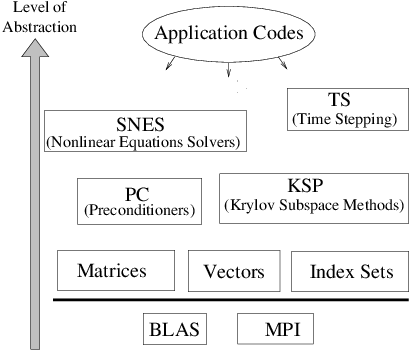
\includegraphics{petscwww}}
%\centerline{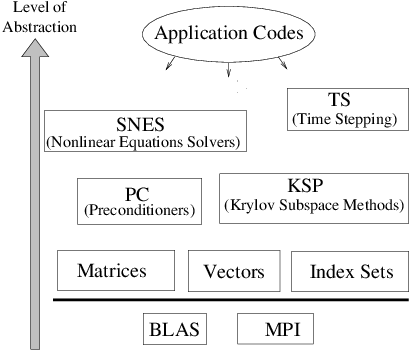
\psfig{file=petscwww.ps,angle=270,height=3.4in}}
% \centerline{\psfig{file=petsc_pt.eps,angle=0,height=4in,width=5in}}
\caption{Organization of the PETSc Libraries}
\label{fig_1}
\end{figure}

\begin{figure}[hbt]
\centerline{ 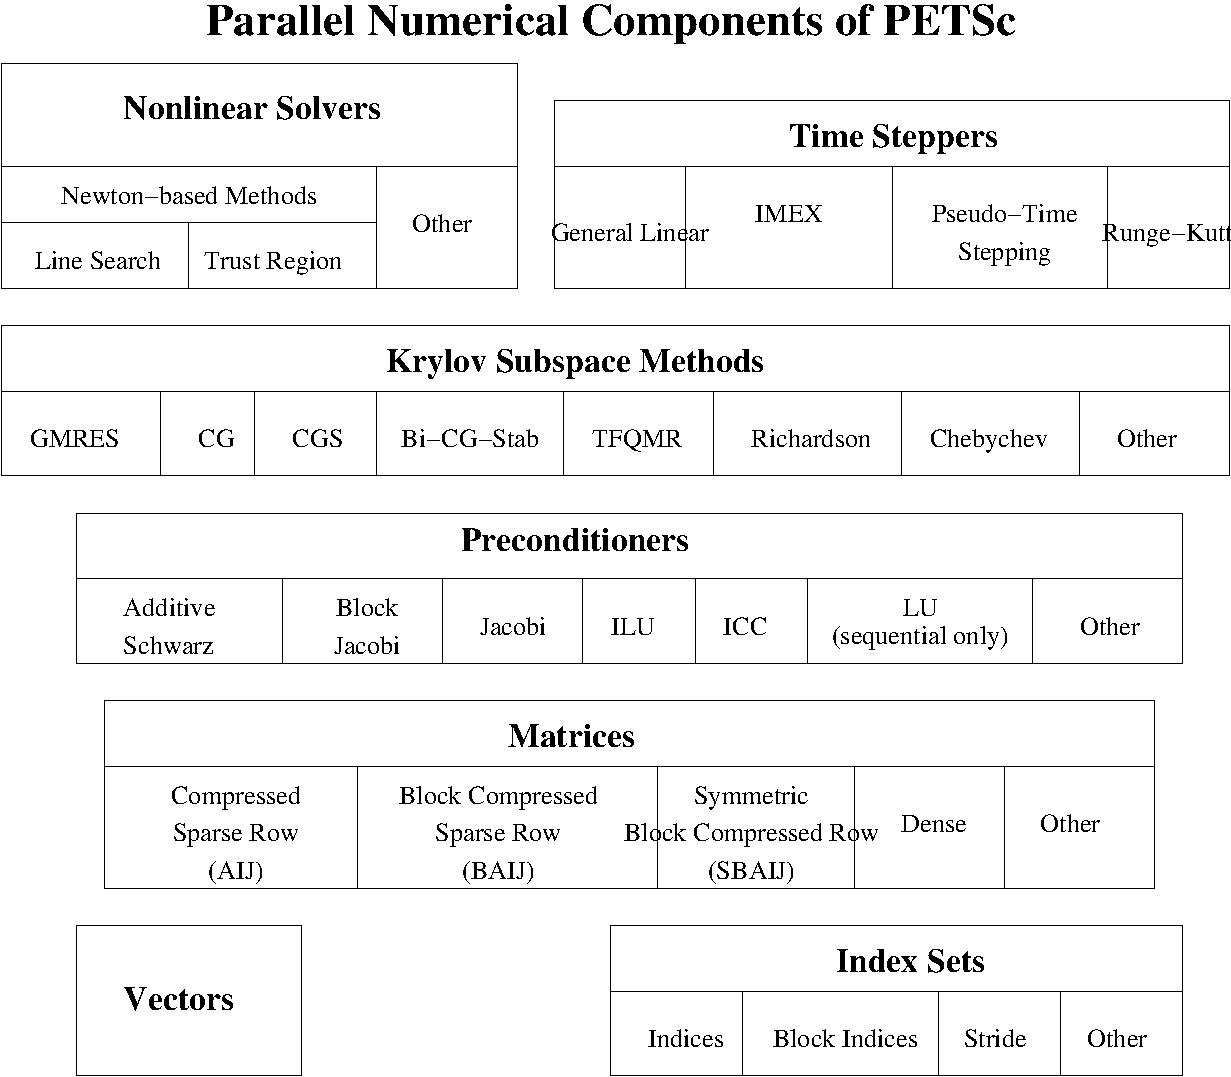
\includegraphics{zoom}}
%\centerline{\psfig{file=zoom_ls.ps,angle=270,height=3.4in}}
\caption{Numerical Libraries of PETSc}
\label{fig_2}
\end{figure}

\section{Suggested Reading}

The manual is
divided into three parts:
\begin{itemize}
\item Part I - Introduction to PETSc
\item Part II - Programming with PETSc
\item Part III - Additional Information
\end{itemize}

Part I describes
the basic procedure for using the PETSc library and presents two
simple examples of solving linear systems with PETSc.  This section
conveys the typical style used throughout the library and enables the
application programmer to begin using the software immediately.
Part I is also distributed separately for individuals interested in an 
overview of the PETSc software, excluding the details of library usage.
Readers of this separate distribution of Part I should note that all
references within the text to particular chapters and sections 
indicate locations in the complete users manual.

Part II explains in detail the use of the various PETSc libraries,
such as vectors, matrices, index sets, linear and nonlinear
solvers, and graphics.  Part III describes a variety of useful
information, including profiling, the options database, viewers, error
handling, makefiles, and some details of
PETSc design.

\nocite{efficient}

PETSc has evolved to become quite a comprehensive package, and therefore the
{\em PETSc Users Manual} can be rather intimidating for new users. We
recommend that one initially read the entire document before proceeding with
serious use of PETSc, but bear in mind that PETSc can be used efficiently
before one understands all of the material presented here. Furthermore, the
definitive reference for any PETSc function is always the online manualpage.

\medskip \medskip

Within the PETSc distribution, the directory \trl{${PETSC_DIR}/docs}
contains all documentation.
Manual pages for all PETSc functions can be
accessed on line at
\begin{tabbing}
  http://www.mcs.anl.gov/petsc/docs/
\end{tabbing}
The manual pages
provide hyperlinked indices (organized by
both concepts and routine names) to the tutorial examples and enable
easy movement among related topics.  

Emacs users may find the
{\em etags} option to be extremely useful for exploring the PETSc
source code.  Details of this feature are provided in
Section~\ref{sec_emacs}. 

The file \trl{manual.pdf} contains
the complete {\em PETSc Users Manual} in the portable document format (PDF), 
while \trl{intro.pdf} 
includes only the introductory segment, Part I.  \sindex{installing PETSc} 
The complete PETSc distribution, users
manual, manual pages, and additional information are also available via
the PETSc home page at
\trllink{http://www.mcs.anl.gov/petsc}{http://www.mcs.anl.gov/petsc}.  
The PETSc home page also
contains details regarding installation, new features and changes in recent
versions of PETSc, machines that we currently support, a
troubleshooting guide, and a FAQ list for frequently asked questions.

\medskip\medskip

\noindent{\bf Note to Fortran Programmers}: In most of the  
manual, the examples and calling sequences are given for the C/C++
family of programming languages.  We follow this convention because we
recommend that PETSc applications be coded in C or C++.
However, pure Fortran programmers can use most of the
functionality of PETSc from Fortran, with only minor differences in
the user interface.  Chapter \ref{ch_fortran} provides a discussion of the
differences between using PETSc from Fortran and C, as well as several
complete Fortran examples.  This chapter also introduces some
routines that support direct use of Fortran90 pointers.

%-----------------------------------------------------------------------------
\section{Running PETSc Programs}
\label{sec_running}

Before using PETSc, the user must first set the environmental variable
\trl{PETSC_DIR}, \findex{PETSC_DIR} indicating the full path of the PETSc home
directory.  For example, under the UNIX C shell a command of the form
\begin{tabbing}
   setenv PETSC\_DIR \$HOME/petsc
\end{tabbing}
 can be placed in the user's \trl{
.cshrc} file.  In addition, the user must set the environmental
variable {\trl{PETSC_ARCH}} to specify the architecture (e.g., rs6000,
solaris, IRIX, etc.)  on which PETSc is being used.  The utility
 \trl{${PETSC_DIR}/bin/petscarch} can be used for this purpose.  For example,
\begin{tabbing}
   setenv PETSC\_ARCH `\$PETSC\_DIR/bin/petscarch`
\end{tabbing}
can be placed in a \trl{.cshrc} file.  Thus, even if several machines of different
types share the same filesystem, \trl{PETSC_ARCH} will be set correctly
when logging into any of them. 

All PETSc programs use the MPI (Message Passing Interface) standard
for message-passing communication \cite{MPI-final}.  Thus, to execute
PETSc programs, users must know the procedure for beginning MPI jobs
on their selected computer system(s).  For instance, when using the
MPICH implementation of MPI \cite{mpich-web-page} and many others, the following
command initiates a program that uses eight processors:
\findex{mpirun} \sindex{running PETSc programs} 
\begin{tabbing}
   mpirun -np 8 petsc\_program\_name petsc\_options
\end{tabbing}

PETSc also comes with a script 
\begin{tabbing}
   \${PETSC\_DIR}/bin/petscmpirun -np 8 petsc\_program\_name petsc\_options
\end{tabbing}
that uses the information set in \trl{${PETSC_DIR}/bmake/${PETSC_ARCH}/packages} to 
automatically use the correct \trl{mpirun} for your configuration.

All PETSc-compliant programs support the use of the \trl{-h}
\findex{-h} or \trl{-help} option as well as the \trl{-v} \findex{-v}
or \trl{-version} option. 


Certain options are supported by all PETSc programs.  We list a few 
particularly useful ones below; a complete list can be obtained by 
running any PETSc program with the option \trl{-help}.
\begin{itemize}
\item \trl{-log_summary} - summarize the program's performance
\item \trl{-fp_trap} - stop on floating-point exceptions; \findex{-fp_trap}
      for example divide by zero
\item \trl{-trdump} - enable memory tracing; dump list of unfreed memory 
      at conclusion \findex{-trdump} of the run
\item \trl{-trmalloc} - enable memory tracing (by default this is 
      activated for versions of PETSc using BOPT=g*)
\item \trl{-start_in_debugger} \trl{[noxterm,gdb,dbx,xxgdb]} \trl{[-display name]} 
     - start all processes in debugger \findex{-start_in_debugger} \sindex{debugger}
\item \trl{-on_error_attach_debugger}  \trl{[noxterm,gdb,dbx,xxgdb]}
      \trl{[-display name]} - \findex{-on_error_attach_debugger}start debugger only on encountering an error
\end{itemize}
See Section \ref{sec_debugging} for more information on debugging PETSc programs.

%-----------------------------------------------------------------------------
\section{Writing PETSc Programs}
\label{sec_writing}

Most PETSc programs begin with a call to \findex{PetscInitialize()}
\begin{tabbing}
  PetscInitialize(int *argc,char ***argv,char *file,char *help);
\end{tabbing} 
which initializes PETSc and MPI.  The arguments \trl{argc} and 
\trl{argv} are the command line arguments delivered in all C and C++
programs. \sindex{command line arguments} The argument \trl{file}
optionally indicates an alternative name for the PETSc options file,
\trl{.petscrc}, which resides by default in the user's home directory.
Section \ref{sec_options} provides details regarding
this file and the PETSc options database, which can be used for runtime
customization. The final argument, \trl{help}, is an optional
character string that will be printed if the program is run with the
\trl{-help} option.  In Fortran the initialization command has the form
\begin{tabbing}
   call PetscInitialize(character(*) file,integer ierr)
\end{tabbing} 
\trl{PetscInitialize()} automatically calls \trl{MPI_Init()} if MPI
has not been not previously initialized. In certain \findex{MPI_Init()}
circumstances in which MPI needs to be initialized directly (or is
initialized by some other library), the user can first call 
\trl{MPI_Init()} (or have the other library do it), and then call
\trl{PetscInitialize()}.
By default, \trl{PetscInitialize()} sets the PETSc ``world''
communicator, given by \trl{PETSC_COMM_WORLD}, to \trl{MPI_COMM_WORLD}.
\findex{PETSC_COMM_WORLD}

For those not familar with MPI, a {\em communicator} is a way of
indicating a collection of processes that will be involved together
in a calculation or communication. Communicators have the variable type
\trl{MPI_Comm}. In most cases users can employ the communicator \trl{
PETSC_COMM_WORLD} to indicate all processes in a given run and \trl{
PETSC_COMM_SELF} to indicate a single process.
\findex{PETSC_COMM_SELF}

MPI provides routines
for generating new communicators consisting of subsets of processors,
though most users rarely need to use these. The book {\em Using MPI},
by Lusk, Gropp, and Skjellum \cite{using-mpi} provides an excellent
introduction to the concepts in MPI, see also the MPI homepage 
\trllink{http://www.mcs.anl.gov/mpi/}{http://www.mcs.anl.gov/mpi/}.
Note that PETSc users need not program much message passing directly
with MPI, but they must be familar with the basic concepts of message
passing and distributed memory computing.

All PETSc routines return an integer indicating whether an error has
occurred during the call.  The error code is set to be nonzero if an
error has been detected; otherwise, it is zero.  For the C/C++
interface, the error variable is the routine's return value, while for
the Fortran version, each PETSc routine has as its final argument an
integer error variable.  Error tracebacks are discussed in the following
section.

All PETSc programs should call \trl{PetscFinalize()} \findex{PetscFinalize()}
as their final (or nearly final) statement, as given below in the C/C++
and Fortran formats, respectively:
\begin{tabbing}
  PetscFinalize();\\
  call PetscFinalize(ierr)
\end{tabbing}
This routine handles options to be called at the conclusion of
the program, and calls \trl{MPI_Finalize()} \findex{MPI_Finalize()}
if \trl{PetscInitialize()}
began MPI. If MPI was initiated externally from PETSc (by either
the user or another software package), the user is
responsible for calling \trl{MPI_Finalize()}. 

\section{Simple PETSc Examples}

\label{sec_simple}

To help the user start using PETSc immediately, we begin with a simple
uniprocessor example in Figure~\ref{fig_example1} that solves the
one-dimensional Laplacian problem with finite differences.  This
sequential code, which can be found in 
\trl{${PETSC_DIR}/src/ksp/examples/tutorials/ex1.c},
illustrates the solution of a linear system with KSP, the 
interface to the preconditioners, Krylov subspace methods, and direct
linear solvers of PETSc.  Following the code we highlight a few of the most important
parts of this example.  

\begin{figure}[H]
{\footnotesize
\fileinclude{../../../src/ksp/examples/tutorials/ex1.c}
}
\caption{Example of Uniprocessor PETSc Code}
\label{fig_example1}
\end{figure}

\subsection*{Include Files}

The C/C++ include files for PETSc should be used via statements such as
\begin{tabbing}
{\footnotesize
   \#include "petscksp.h"
}
\end{tabbing}
where \trl{petscksp.h} is the include file for the linear solver library.
Each PETSc program must specify an
include file that corresponds to the highest level PETSc objects
needed within the program; all of the required lower level include
files are automatically included within the higher level files.  For
example, \trl{petscksp.h} includes \trl{petscmat.h} (matrices),
\trl{petscvec.h} (vectors), and \trl{petsc.h} (base PETSc file).  
The PETSc include files are located in the directory 
\trl{${PETSC_DIR}/include}.  See Section \ref{sec_fortran_includes}
for a discussion of PETSc include files in Fortran programs.

\subsection*{The Options Database}

As shown in Figure~\ref{fig_example1}, the user can input control data
at run time using the options database. In this example the command
\trl{PetscOptionsGetInt(PETSC_NULL,"-n",&n,&flg);} checks whether the user has
provided a command line option to set the value of \trl{n}, the
problem dimension.  If so, the variable \trl{n} is set accordingly;
otherwise, \trl{n} remains unchanged. A complete description of the
options database may be found in Section \ref{sec_options}.

\subsection*{Vectors}
\label{sec_vecintro}

One creates a new parallel or 
sequential vector, \trl{x}, of global dimension \trl{M} with the 
commands \findex{VecCreate()}  \findex{VecSetSizes()} \sindex{vectors}
\begin{tabbing}
  VecCreate(MPI\_Comm comm,Vec *x);
  VecSetSizes(Vec x, int m, int M);
\end{tabbing}
where \trl{comm} denotes the MPI communicator and \trl{m} is the optional local size
which may be \trl{PETSC_DECIDE}. The type of storage
for the vector may be set with either calls to 
\trl{VecSetType()} or \trl{VecSetFromOptions()}. \findex{VecSetType()} \findex{VecSetFromOptions()}
Additional vectors of the same type can be formed with
\findex{VecDuplicate()}
\begin{tabbing}
  VecDuplicate(Vec old,Vec *new);
\end{tabbing}
The commands \findex{VecSet()} \findex{VecSetValues()}
\begin{tabbing}
  VecSet(PetscScalar *value,Vec x);\\
  VecSetValues(Vec x,int n,int *indices,PetscScalar *values,INSERT\_VALUES);
\end{tabbing}
respectively set all the components of a vector to a particular scalar
value and assign a different value to each component.  More
detailed information about PETSc vectors, including their basic
operations, scattering/gathering, index sets, and distributed arrays, is
discussed in Chapter~\ref{chapter_vectors}.

\findex{PetscScalar} \sindex{complex numbers}
Note the use of the PETSc variable type \trl{PetscScalar} in this example.
The \trl{PetscScalar} is simply defined to be \trl{double} in C/C++
(or correspondingly \trl{double} \trl{precision} in Fortran) for versions of
PETSc that have {\em not} been compiled for use with complex numbers.
The \trl{PetscScalar} data type enables
identical code to be used when the PETSc libraries have been compiled
for use with complex numbers.  Section~\ref{sec_complex} discusses the
use of complex numbers in PETSc programs.

\subsection*{Matrices}
\label{sec_matintro}

Usage of PETSc matrices and vectors is similar. \sindex{matrices} 
The user can create a new parallel or sequential matrix, \trl{A}, which
has \trl{M} global rows and \trl{N} global columns, with the routine
\findex{MatCreate()}
\begin{tabbing}
  MatCreate(MPI\_Comm comm,int m,int n,int M,int N,Mat *A);
\end{tabbing}
where the matrix format can be specified at runtime.  The user could
alternatively specify each processes' number of local rows and columns
using \trl{m} and \trl{n}.
Values can then be set with the command
\begin{tabbing}
  MatSetValues(Mat A,int m,int *im,int n,int *in,PetscScalar *values,INSERT\_VALUES);
\end{tabbing}
After \findex{MatSetValues()} all elements have been inserted into the
matrix, it must be processed with the pair of commands
\findex{MatAssemblyBegin()} \findex{MatAssemblyEnd()}
\begin{tabbing}
  MatAssemblyBegin(Mat A,MAT\_FINAL\_ASSEMBLY);\\
  MatAssemblyEnd(Mat A,MAT\_FINAL\_ASSEMBLY);
\end{tabbing}
Chapter~\ref{chapter_matrices} discusses various matrix formats as
well as the details of some basic matrix manipulation routines.

\subsection*{Linear Solvers}

After creating the matrix and vectors that define a linear system,
\trl{Ax = b}, the user can then use KSP to solve the system 
with the following sequence of commands: 
\findex{KSPCreate()} \findex{KSPSetOperators()}
\findex{KSPSetFromOptions()} \findex{KSPSolve()} \findex{KSPDestroy()}
\begin{tabbing}
  KSPCreate(MPI\_Comm comm,KSP *ksp); \\
  KSPSetOperators(KSP ksp,Mat A,Mat PrecA,MatStructure flag);\\
  KSPSetFromOptions(KSP ksp);\\
  KSPSolve(KSP ksp,Vec b,Vec x);\\
  KSPDestroy(KSP ksp);
\end{tabbing}
The user first creates the KSP context and sets the operators
associated with the system (linear system matrix and optionally different
preconditioning matrix).  The user then sets various options for
customized solution, solves the linear system, and finally destroys
the KSP context.  We emphasize the command \trl{KSPSetFromOptions()}, 
which enables the user to customize the linear solution
method at runtime by using the options database, which is discussed in
Section~\ref{sec_options}. Through this database, the user not only
can select an iterative method and preconditioner, but also can prescribe
the convergence tolerance, set various monitoring routines, etc.
(see, e.g., Figure~\ref{fig_exprof}).

Chapter~\ref{ch_ksp} describes in detail the KSP package, including
the PC and KSP packages for preconditioners and Krylov subspace methods.

\subsection*{Nonlinear Solvers}
Most PDE problems of interest are inherently nonlinear. PETSc provides 
an interface to tackle the nonlinear problems directly called SNES. Chapter
\ref{chapter_snes} describes the nonlinear solvers in detail. We recommend 
most PETSc users work directly with SNES, rather than using PETSc
for the linear problem within a nonlinear solver.

\subsection*{Error Checking}

All PETSc routines return an integer indicating whether an error
has occurred during the call.  The PETSc macro \trl{CHKERRQ(ierr)}
checks the value of \trl{ierr} and calls the PETSc error handler
upon error detection.  \trl{CHKERRQ(ierr)} should be used in all
subroutines to enable a complete error traceback.
In Figure~\ref{fig_traceback} we indicate a
traceback generated by error detection within a sample PETSc
program. The error occurred on line 1673 of the file \trl{
${PETSC_DIR}/src/mat/impls/aij/seq/aij.c} and was caused by trying to allocate too
large an array in memory. The routine was called in the program 
\trl{ex3.c} on line 71.  See Section \ref{sec_fortran_errors} for
details regarding error checking when using the PETSc Fortran interface.

\begin{figure}[H]
\begin{tabbing}
   eagle:mpirun -np 1 ex3 -m 10000\\
   PETSC ERROR: MatCreateSeqAIJ() line 1673 in src/mat/impls/aij/seq/aij.c\\
   PETSC ERROR:   Out of memory. This could be due to allocating\\
   PETSC ERROR:   too large an object or bleeding by not properly\\
   PETSC ERROR:   destroying unneeded objects.\\
   PETSC ERROR:   Try running with -trdump for more information.\\ 
   PETSC ERROR: MatCreate() line 99 in src/mat/utils/gcreate.c  \\
   PETSC ERROR: main() line 71 in src/ksp/examples/tutorials/ex3.c\\  
   MPI Abort by user Aborting program !\\
   Aborting program! \\
   p0\_28969:  p4\_error: : 1
\end{tabbing}
\nobreak
\caption{Example of Error Traceback}
\label{fig_traceback}
\end{figure}

When running the debug (BOPT=g compiled) version of the PETSc libraries, it
does a great deal of checking for memory corruption (writing outside of 
array bounds etc). The macros \trl{CHKMEMQ} can be called 
anywhere in the code to check the current status of the memory for corruption.
By putting several (or many) of these macros into your code you can usually 
easily track down in what small segment of your code the corruption has occured.

\subsection*{Parallel Programming}

Since PETSc uses the message-passing model for
parallel programming and employs MPI for all interprocessor
communication, the user is free to employ MPI routines as needed
throughout an application code.  However, by default the user is
shielded from many of the details of message passing within PETSc,
since these are hidden within parallel objects, such as vectors,
matrices, and solvers.  In addition, PETSc provides tools such as
generalized vector scatters/gathers and distributed arrays to assist
in the management of parallel data.

\sindex{collective operations}
Recall that the user must specify a communicator upon creation of any
PETSc object (such as a vector, matrix, or solver) to indicate the
processors over which the object is to be distributed.  For example,
as mentioned above, some commands for matrix, vector, and linear solver
creation are:
\begin{tabbing}
  MatCreate(MPI\_Comm comm,int M,int N,Mat *A);\\
  VecCreate(MPI\_Comm comm,Vec *x);\\
  KSPCreate(MPI\_Comm comm,KSP *ksp); 
\end{tabbing}
The creation routines are collective over all processors in the
communicator; thus, all processors in the communicator {\em must}
call the creation routine.  In addition, if a sequence of
collective routines is being used, they {\em must} be called
in the same order on each processor.

The next example, given in Figure~\ref{fig_example2}, illustrates the
solution of a linear system in parallel.  This code, corresponding to
\trl{${PETSC_DIR}/src/ksp/examples/tutorials/ex2.c}, handles the
two-dimensional Laplacian discretized with finite differences, where
the linear system is again solved with KSP.  The code performs the
same tasks as the sequential version within Figure~\ref{fig_example1}.
Note that the user interface for initiating the program, creating
vectors and matrices, and solving the linear system is {\em exactly}
the same for the uniprocessor and multiprocessor examples.  The
primary difference between the examples in Figures \ref{fig_example1}
and \ref{fig_example2} is that each processor forms only its local
part of the matrix and vectors in the parallel case.

\begin{figure}[H]
{\footnotesize
\fileinclude{../../../src/ksp/examples/tutorials/ex2.c}
}
\nobreak
\caption{Example of Multiprocessor PETSc Code}
\label{fig_example2}
\end{figure}

\subsection*{Compiling and Running Programs}

Figure~\ref{fig_exrun} illustrates compiling and running a PETSc program
using MPICH.  Note that different sites may have slightly different
library and compiler names.  See Chapter \ref{ch_makefiles}
for a discussion about compiling PETSc programs.
Users who are experiencing difficulties linking PETSc programs should 
refer to the troubleshooting guide via the PETSc WWW home page 
\trllink{http://www.mcs.anl.gov/petsc}{http://www.mcs.anl.gov/petsc} or
given in the file \trllink{troubleshooting.html}{${PETSC_DIR}/docs/troubleshooting.html}.

\begin{figure}[H]
{\small
\begin{tabbing}
   eagle: make BOPT=g ex2\\
   gcc  -pipe -c  -I../../../  -I../../..//include   \\
       -I/usr/local/mpi/include  -I../../..//src -g \\
       -DPETSC\_USE\_DEBUG -DPETSC\_MALLOC -DPETSC\_USE\_LOG ex1.c\\
   gcc -g -DPETSC\_USE\_DEBUG -DPETSC\_MALLOC -DPETSC\_USE\_LOG -o ex1 ex1.o \\
      /home/bsmith/petsc/lib/libg/sun4/libpetscksp.a \\
      -L/home/bsmith/petsc/lib/libg/sun4 -lpetscstencil -lpetscgrid  -lpetscksp \\
      -lpetscmat  -lpetscvec -lpetscsys -lpetscdraw  \\
      /usr/local/lapack/lib/lapack.a /usr/local/lapack/lib/blas.a \\
      /usr/lang/SC1.0.1/libF77.a -lm /usr/lang/SC1.0.1/libm.a -lX11 \\
      /usr/local/mpi/lib/sun4/ch\_p4/libmpi.a\\
      /usr/lib/debug/malloc.o /usr/lib/debug/mallocmap.o  \\
      /usr/lang/SC1.0.1/libF77.a -lm /usr/lang/SC1.0.1/libm.a -lm\\
   rm -f ex1.o\\
   eagle: mpirun -np 1 ex2\\
   Norm of error 3.6618e-05 iterations 7\\
   eagle:\\
   eagle: mpirun -np 2 ex2\\
   Norm of error 5.34462e-05 iterations 9
\end{tabbing}
}
\nobreak
\caption{Running a PETSc Program}
\label{fig_exrun}
\end{figure}

As shown in Figure \ref{fig_exprof}, the option \trl{
-log_summary} activates printing of a performance summary, including
times, floating point operation (flop) rates, and message-passing
activity.  Chapter~\ref{ch_profiling}
provides details about profiling, including interpretation of the
output data within Figure~\ref{fig_exprof}.  This particular example involves the solution of a linear
system on one processor using GMRES and ILU.  The low floating point
operation (flop) rates in this example are due to the fact that the
code solved a tiny system.  We include this example merely to
demonstrate the ease of extracting performance information.

\begin{figure}[H]
{\footnotesize
\begin{verbatim}
eagle> mpirun -np 1 ex1 -n 1000 -pc_type ilu -ksp_type gmres -ksp_rtol 1.e-7 -log_summary
-------------------------------- PETSc Performance Summary: --------------------------------------

ex1 on a sun4 named merlin.mcs.anl.gov with 1 processor, by curfman Wed Aug  7 17:24:27 1996

                         Max         Min        Avg        Total 
Time (sec):           1.150e-01      1.0   1.150e-01
Objects:              1.900e+01      1.0   1.900e+01
Flops:                3.998e+04      1.0   3.998e+04  3.998e+04
Flops/sec:            3.475e+05      1.0              3.475e+05
MPI Messages:         0.000e+00      0.0   0.000e+00  0.000e+00
MPI Messages:         0.000e+00      0.0   0.000e+00  0.000e+00 (lengths)
MPI Reductions:       0.000e+00      0.0

--------------------------------------------------------------------------------------------------
Phase             Count      Time (sec)       Flops/sec                             -- Global --    
                            Max     Ratio    Max    Ratio   Mess  Avg len  Reduct  %T %F %M %L %R   
--------------------------------------------------------------------------------------------------
MatMult               2  2.553e-03    1.0  3.9e+06    1.0  0.0e+00 0.0e+00 0.0e+00  2 25  0  0  0
MatAssemblyBegin      1  2.193e-05    1.0  0.0e+00    0.0  0.0e+00 0.0e+00 0.0e+00  0  0  0  0  0
MatAssemblyEnd        1  5.004e-03    1.0  0.0e+00    0.0  0.0e+00 0.0e+00 0.0e+00  4  0  0  0  0
MatGetReordering      1  3.004e-03    1.0  0.0e+00    0.0  0.0e+00 0.0e+00 0.0e+00  3  0  0  0  0
MatILUFctrSymbol      1  5.719e-03    1.0  0.0e+00    0.0  0.0e+00 0.0e+00 0.0e+00  5  0  0  0  0
MatLUFactorNumer      1  1.092e-02    1.0  2.7e+05    1.0  0.0e+00 0.0e+00 0.0e+00  9  7  0  0  0
MatSolve              2  4.193e-03    1.0  2.4e+06    1.0  0.0e+00 0.0e+00 0.0e+00  4 25  0  0  0
MatSetValues       1000  2.461e-02    1.0  0.0e+00    0.0  0.0e+00 0.0e+00 0.0e+00 21  0  0  0  0
VecDot                1     60e-04    1.0  9.7e+06    1.0  0.0e+00 0.0e+00 0.0e+00  0  5  0  0  0
VecNorm               3  5.870e-04    1.0  1.0e+07    1.0  0.0e+00 0.0e+00 0.0e+00  1 15  0  0  0
VecScale              1  1.640e-04    1.0  6.1e+06    1.0  0.0e+00 0.0e+00 0.0e+00  0  3  0  0  0
VecCopy               1  3.101e-04    1.0  0.0e+00    0.0  0.0e+00 0.0e+00 0.0e+00  0  0  0  0  0
VecSet                3  5.029e-04    1.0  0.0e+00    0.0  0.0e+00 0.0e+00 0.0e+00  0  0  0  0  0
VecAXPY               3  8.690e-04    1.0  6.9e+06    1.0  0.0e+00 0.0e+00 0.0e+00  1 15  0  0  0
VecMAXPY              1  2.550e-04    1.0  7.8e+06    1.0  0.0e+00 0.0e+00 0.0e+00  0  5  0  0  0
KSPSolve             1  1.288e-02    1.0  2.2e+06    1.0  0.0e+00 0.0e+00 0.0e+00 11 70  0  0  0
KSPSetUp             1  2.669e-02    1.0  1.1e+05    1.0  0.0e+00 0.0e+00 0.0e+00 23  7  0  0  0
KSPGMRESOrthog        1  1.151e-03    1.0  3.5e+06    1.0  0.0e+00 0.0e+00 0.0e+00  1 10  0  0  0
PCSetUp               1 24e-02    1.0  1.5e+05    1.0  0.0e+00 0.0e+00 0.0e+00 18  7  0  0  0
PCApply               2  4.474e-03    1.0  2.2e+06    1.0  0.0e+00 0.0e+00 0.0e+00  4 25  0  0  0
-------------------------------------------------------------------------------------------------

Memory usage is given in bytes:

Object Type      Creations   Destructions   Memory  Descendants' Mem.
Index set             3              3      12420     0
Vector                8              8      65728     0
Matrix                2              2     184924     4140
Krylov Solver         1              1      16892     41080
Preconditioner        1              1          0     64872
KSP                  1              1          0     122844

\end{verbatim}
}
\nobreak
\caption{Running a PETSc Program with Profiling}
\label{fig_exprof}
\end{figure}

\subsection*{Writing Application Codes with PETSc}

The examples throughout the library demonstrate the software usage
and can serve as templates for developing
custom applications.  We suggest that new PETSc
users examine programs in the directories 
\begin{tabbing}
  \trl{${PETSC_DIR}/src/<library>/examples/tutorials},
\end{tabbing}
where \trl{<library>}
denotes any of the PETSc libraries (listed in the following
section), such as \trl{snes} or \trl{ksp}.  
The manual pages located at
\begin{tabbing}
   \${PETSC\_DIR}/docs/index.html or \\
   http://www.mcs.anl.gov/petsc/docs/
\end{tabbing}
provide indices (organized by both routine names and concepts) to the tutorial examples.

To write a new application program using PETSc, we suggest the
following procedure:
\begin{enumerate}
\item Install and test PETSc according to the instructions at the PETSc web site.
\item Copy one of the many PETSc examples in the directory
      that corresponds to the class of problem of interest (e.g.,
      for linear solvers, see \trl{${PETSC_DIR}/src/ksp/examples/tutorials}).
\item Copy the corresponding makefile within the example directory;
      compile and run the example program.
\item Use the example program as a starting point for developing a custom code.
\end{enumerate}

%---------------------------------------------------------------------

\section{Referencing PETSc}

When referencing PETSc in a publication please cite the following:
\begin{tabbing}
@Unpublished\{petsc-home-page,\\
   Author = "Satish Balay and William D. Gropp and Lois C. McInnes and Barry F. Smith",\\
   Title  = "PETSc home page",\\
   Note   = "http://www.mcs.anl.gov/petsc",\\
   Year   = "2001"\}\\

@TechReport\{petsc-manual,\\
   Author      = "Satish Balay and William D. Gropp and Lois C. McInnes and Barry F. Smith",\\
   Title       = "PETSc Users Manual",\\
   Number      = "ANL-95/11 - Revision 2.1.5",\\
   Institution = "Argonne National Laboratory",\\
   Year        = "2003"\}\\

@InProceedings\{petsc-efficient,\\
   Author    = "Satish Balay and William D. Gropp and Lois C. McInnes and Barry F. Smith",\\
   Title     = "Efficienct Management of Parallelism in Object Oriented Numerical Software Libraries",\\
   Booktitle = "Modern Software Tools in Scientific Computing",\\
   Editor    = "E. Arge and A. M. Bruaset and H. P. Langtangen",\\
   Pages     = "163--202",\\
   Publisher = "Birkhauser Press",\\
   Year      = "1997"\}
\end{tabbing}


%---------------------------------------------------------------------

\section{Directory Structure}

We conclude this introduction with an overview of the
organization of the PETSc software.  
The root directory of PETSc contains the following directories:
% As shown in Figure~\ref{fig_directories}, the root directory of PETSc contains the following directories:

\begin{itemize}
\item \trl{docs} - All documentation for PETSc. The files \trl{manual.pdf}
                   contains the hyperlinked users manual, suitable for printing
                   or on-screen viewering. Includes the subdirectory
 \subitem - \trl{manualpages} (on-line manual pages).
\item \trl{bin} - Utilities and short scripts for use with PETSc, including
 \begin{itemize}
 \item \trl{petsarch} (utility for setting \trl{PETSC_ARCH} environmental variable),
 \end{itemize}

\item \trl{bmake} - Base PETSc makefile directory.  Includes subdirectories
                    for various architectures.
\item \trl{include} - All include files for PETSc that are visible to the user.
\item \trl{include/finclude}    - PETSc include files for Fortran programmers using 
                                  the .F suffix (recommended).
\item \trl{include/pinclude}    - Private PETSc include files that should {\em not} 
                                  be used by application programmers.
\item \trl{src} - The source code for all PETSc libraries, which
                  currently includes
 \begin{itemize}
 \item \trl{vec} - vectors,
   \begin{itemize}
     \item \trl{is} - index sets,
   \end{itemize}
 \item \trl{mat} - matrices,
 \item \trl{dm}
   \begin{itemize}
    \item \trl{da} - distributed arrays,
    \item \trl{ao} - application orderings,
   \end{itemize}
 \item \trl{ksp} - complete linear equations solvers,
 \begin{itemize}
   \item \trl{ksp} - Krylov subspace accelerators,
   \item \trl{pc} - preconditioners,
 \end{itemize}
 \item \trl{snes} - nonlinear solvers
 \item \trl{ts} - ODE solvers and timestepping,
 \item \trl{sys} - general system-related routines,
 \begin{itemize}
   \item \trl{plog} - PETSc logging and profiling routines,
   \item \trl{draw} - simple graphics,
 \end{itemize}
 \item \trl{fortran} - Fortran interface stubs,
 \item \trl{contrib} - contributed modules that use PETSc but are not
    part of the official PETSc package.  We encourage users who have
    developed such code that they wish to share with others to let us
    know by writing to petsc-maint@mcs.anl.gov.
 \end{itemize}
\end{itemize}

Each PETSc source code library directory has the following subdirectories:
\begin{itemize}
\item  \trl{examples} - Example programs for the component, including
  \begin{itemize}
  \item \trl{tutorials} - Programs designed to teach users about PETSc.  These
          codes can serve as templates for the design of custom applicatinos.
  \item \trl{tests} - Programs designed for thorough testing of PETSc.  As such,
          these codes are not intended for examination by users.
  \end{itemize}
\item  \trl{interface} - The calling sequences for the abstract interface  
        to the component.
        Code here does not know about particular implementations.
\item  \trl{impls} - Source code for one or more implementations.
\item  \trl{utils} - Utility routines.  Source here may know about the 
          implementations, but ideally will not know about implementations
          for other components.
\end{itemize}

%
% Picture is not up to date, so temporarily exclude this.
%
% \begin{figure}[tb]
% \centerline{\psfig{file=dirs.ps,angle=270,height=6in,width=6in}}
% \nobreak
% \caption{Schematic of the PETSc Directory Structure}
% \label{fig_directories}
% \end{figure}


% ------------------------------------------------------------------
%   End of introductory information
% ------------------------------------------------------------------


\end{document}

\section{Bound-Constrained Quadratic Optimization Problem}

\label{qp}

We assume that the quadratic $q : \R^n \mapsto \R $ is strictly convex
on the feasible region
\begin{equation} \label{def_bounds}
\Omega = \{ x \in \R^n: l \leq x \leq u \} .
\end{equation}
This assumption guarantees that the bound-constrained 
quadratic optimization problem (\ref{def_bqp}) has a unique solution
in  $\Omega$.
Also note that since $q$ is strictly convex, we can define
\begin{equation} \label{def-quadratic}
q(x) = \half \langle x , {A} x \rangle + \langle b , x \rangle + c,
\end{equation}
where $A \in \R^{n \times n}$ is symmetric and
positive definite, $ b \in \R^n$, and $c \in \R$.

We allow the feasible set \Ref{def_bounds} to be unbounded,
and thus the components of $l$ or $u$ can be infinite.
We also allow variables to be fixed by setting $ l_i = u_i $.
If $ l_i < u_i $, then  solutions to problem \Ref{def_bqp} 
satisfy the Kuhn-Tucker conditions
\[ \begin{array}{lllll}
\partial_iq(x) & = & 0 & \mbox{ if } & x_i \in (l_i, u_i) \\
\partial_iq(x) & \geq & 0 & \mbox{ if } & x_i = l_i \\
\partial_iq(x) & \leq & 0 & \mbox{ if } & x_i = u_i , \\
\end{array}
\]
where $\partial_iq(x)$ is the partial derivative of $q$ with
respect to the $i$th variable.
Approximate solutions can be defined in terms of the projected
gradient, defined by
\begin{equation} \label{proj-gradient}
 \left[ \nabla _{\Omega} q(x) \right] _i = \left\{
\begin{array}{lll}
\partial_i q(x) & \mbox{ if } & x_i \in (l_i, u_i) \\
\min \{ \partial_i q(x),0 \} & \mbox{ if } & x_i = l_i \\
\max \{ \partial_i q(x),0 \} & \mbox{ if } & x_i = u_i .
\end{array}
\right.
\end{equation}
This definition of a projected gradient is appropriate 
% for the bound constrained problem (\ref{def_bqp}) 
because $x^*$ is a solution of (\ref{def_bqp}) if and only if
$\nabla_{\Omega} q(x^*)=0$.

Given $x_0 \in \Omega$, and a tolerance $\tau$, an
approximate solution to the bound constrained problem (\ref{def_bqp}) 
is any vector $x \in \Omega$ such
that
\begin{equation} 
\label{bqp_approximate_sol}
\| \nabla_{\Omega} q(x) \| \leq \tau . % \| \grad q(x_0) \| .
\end{equation}
Note that (\ref{bqp_approximate_sol}) holds whenever
$x$ is sufficiently close to $x^*$ and in the face of $\Omega $ that
contains $x^*$.  The concept of a face is standard in convex analysis;
for the convex set (\ref{def_bounds}), the face of $\Omega$ that contains
$x$ is
\[ 
\Bigl \{ v \in \Omega: v_i = x_i \mbox{ if } x_i \in \{ l_i, u_i \} \Bigr \}. 
\]
Thus, the face of the feasible set that contains $x$ can
be described in terms of the set of active constraints
\[ 
{\cal A}(x) = \{ i: x_i = l_i \mbox{ or } x_i = u_i \}. 
\]
Variables with indices in ${\cal A}(x)$ are the active variables,
and those with indices outside  ${\cal A}(x)$ are the free variables.
Similarly, the binding variables are those with indices in
\[ 
{\cal B}(x) = \{ i:x_i=l_i \mbox{ and } \partial_iq(x) \geq 0,
\mbox{ or } x_i=u_i \mbox{ and } \partial_iq(x) \leq 0 \}. 
\]
The Kuhn-Tucker conditions show that 
$ \cB (x) = \cA (x) $ at a solution, so that if all the active
variables are not binding, then $x$ is not on the face
that contains the solution.


\section{The GPCG Algorithm}

\label{alg}

The GPCG algorithm uses a gradient projection method
to identify a face of the feasible region $ \Omega $
that contains the solution, and the conjugate gradient
method to search the face.
This section provides an outline of the algorithm and notes any
differences between our implementation and the implementation
of Mor\'e and Toraldo \cite{more-toraldo}.

Given $y_0=x_k$,
the gradient projection method generates a sequence of vectors $\{y_j\}$
in the feasible region $\Omega$ such that
\begin{equation} \label{next-y}
y_{j+1} = P [ y_j - \alpha_j \nabla q(y_j) ],  
\end{equation}
where $P$ is the projection
onto (\ref{def_bounds}), and
the step size $\alpha_j$ is chosen such that
\begin{equation}  \label{gplsstop}
 q(y_{j+1}) \leq q(y_j) + \mu
\langle \nabla q(y_j), P [ y_j - \alpha_j \nabla q(y_j) ] - y_j \rangle
\end{equation}
for some $\mu \in (0, 1/2 )$.
The projection $P$ can be computed in $n$ operations by
\[ 
P[x] = \mbox{ mid} (l,u,x), 
\]
where $\mbox{ mid} (l,u,x)$ is the vector whose $i${th} component
is the median of the set $\{ l_i, u_i, x_i \} $.
The step size is computed by a
projected search \cite{more-toraldo} by setting $ \alpha_j $
to the first member of the sequence
$ \alpha_0 ( \half ) ^ j $ for $ j = 0, 1, \ldots $ such that
$ y_{j+1} $ satisfies the sufficient decrease condition \Ref{gplsstop}.
In our implementation, we use
\begin{equation} \label{bqpls}
\alpha_{0}= \arg \min 
\left \{ 
q \left (y_j - \alpha  \nabla_{\Omega} q(y_j) \right ):
\alpha > 0 
\right \} .
\end{equation}
Computation of $ \alpha_0 $ is straightforward, since 
the mapping 
$ \alpha \mapsto 
q \left (y_j - \alpha  \nabla_{\Omega} q(y_j) \right ) $ is
a quadratic.

We generate gradient projection
iterates until sufficient progress is not made or
the active set settles down.
Thus, we generate iterates until either
\begin{equation} 
\label{pgstop1}
 {\cal A}(y_j) = {\cal A}(y_{j-1})
\end{equation}
or the condition
\begin{equation} 
\label{pgstop2}
 q(y_{j-1}) - q(y_j) \leq \eta_1 \max \{q(y_{l-1}) - q(y_l) : 1 \leq l < j \},
\end{equation}
holds for some tolerance $ \eta_1 $ in $ (0,1) $.
If either test is satisfied, we proceed to the
conjugate gradient part of the algorithm.

The first test (\ref{pgstop1}) measures when the
active set settles down. For nondegenerate problems, 
(\ref{pgstop1}) holds in a neighborhood of the solution.
The gradient
projection could be followed until the optimal face is found, but
experience has shown that a large number of iterates may be required.
The second test (\ref{pgstop2}) measures when
the gradient projection method is not making sufficient progress.

Given an iterate $x_k$ and the active set  ${\cal A}(x_k)$,
the conjugate gradient method computes an approximate
minimizer to the subproblem
\begin{equation} \label{cg}
\min \{ q(x_k + d): d_i = 0, i \in {\cal A}(x_k) \}.
\end{equation}
This problem is unconstrained in the free variables.  Note that
if $x_k$ lies in the same face as the solution and $d_k$ solves
(\ref{cg}), then $x_k + d_k$ is the solution of (\ref{def_bqp}).

The conjugate gradient algorithm for solving
\Ref {cg} is implemented by expressing
this subproblem in terms of an equivalent subproblem in the
free variables.
Let $ i_1, \ldots, i_{m_k} $
be the indices of the free variables, and let
the matrix $Z_k$ be the matrix in $\R^{n \times m_k} $ whose
$j$th column is the $i_j$th column of the identity matrix in
$\R^{n \times n}$. With this notation we see that
subproblem \Ref{cg} is equivalent to the
unconstrained subproblem
\begin{equation}
\min \{ q _ k ( w ) : w \in \R ^ { m_k } \}  ,
\label{cg2}
\end{equation}
where
\[
q_k(w) \equiv q ( x _ k + Z _ k  w ) - q ( x_k ) =
\half \langle w , {A_k} w \rangle + \langle r_k , w \rangle  .
\]
The matrix $ A_k $ and the vector $ r_k $ are, respectively, the
reduced Hessian matrix of $q$ and reduced gradient of $q$ at $x_k$
with respect to the free variables.
If $A$ is the Hessian matrix of the quadratic $q$, then
\[
A_k = Z_k^T A Z_k , \qquad r_k = Z_k^T \nabla q(x_k)  .
\]
Also note that $A_k$ is the matrix obtained from
$A$ by taking those rows and columns whose indices correspond
to free variables;
similarly, $r_k$ is obtained from $\nabla q(x_k)$ by
taking the components whose indices correspond to free variables.

Given a starting point $ w_0 \in \R^{m_k} $, the conjugate gradient algorithm
generates a sequence of iterates $ w _ 0 , w_1 , \ldots $
that terminates at a solution
of subproblem \Ref {cg2} in at most $m_k$ iterations.
We use the conjugate gradient algorithm 
until it generates $ w _ j $ such that
\begin{equation}
q_k ( w_{j-1} ) - q_k ( w _ {j} ) \le \eta_2 \max \{
q_k ( w_{l-1} ) - q_k ( w _ {l} ) : 1 \le l \lt j \}
\label{cgstop1}
\end{equation}
for some tolerance $ \eta_2 > 0 $. 
The approximate 
solution of \Ref {cg} is then
$ d _ k = Z_k w _ {j_k} $, where $j_k$ is the first index $j$
that satisfies \Ref {cgstop1}.

The termination test \Ref{cgstop1} is not standard.
Iterative solvers usually terminate when
\[
\| r_j + A_j w_j \| \le \eta_2 \|r_j\| 
\]
for some tolerance $\eta_2 \in (0,1) $.
This test suffers from the erratic behavior
of the residual $ \| r_j + A_j w_j \| $.
On the other hand, the termination test \Ref{cgstop1}
depends on  whether the conjugate gradient method
is making sufficient progress.

Given the direction $ d_k $, we use a projected
search \cite{more-toraldo} to define 
$ x_{k+1} = P [ x_k + \alpha_k d_k] $, where
$ \alpha_k $ is the first element in
the sequence $ ( \half ) ^ k $ for $ k = 0, 1, \ldots $ such that
\begin{equation}  \label{cglsstop2}
 q( x_{k+1} ) \le  q(x_k) + \mu
\langle \nabla q(x_k), x_{k+1} - x_k \rangle .
\end{equation}
More sophisticated projected searches are possible \cite{more-toraldo}
,
but this simple search has proved to be sufficient in all cases tried.
If
\begin{equation}
\label{cgstop3}
\cB ( x_{k+1} ) = \cA ( x_{k+1} ) ,
\end{equation}
then we find a more
accurate solution to subproblem \Ref{cg2} by reducing $ \eta_2 $
and continuing with the conjugate gradient method.
Otherwise, we terminate this iteration.

\begin{Algorithm}
\noindent{\bf Algorithm GPCG}
\begin{list}{}
{
\setlength{\parsep}{0pt}
\setlength{\itemsep}{0pt}
\setlength{\topsep}{0pt}
}
\item[]
Choose $ x_0 \in \Omega $.
\item[]
For $ k = 0, \ldots, $
\begin{list}{$\bullet$}
{
% \setlength{\parsep}{0pt}
% \setlength{\itemsep}{0pt}
% \setlength{\topsep}{0pt}
}
\item[]
Set $y_0 = x_k$, and generate gradient projection iterates
$y_1, \ldots, y_{j_k}$, where $j_k$ is the first index to satisfy
(\ref{pgstop1}) or (\ref{pgstop2}). 
Set $x_k= y_{j_k}$.

\item[]
Set $ w_0 = 0 $, and
generate conjugate gradient iterates $ w_1 , \ldots, w_{j_k} $
for the reduced system (\ref{cg}).
Set $ d _ k = Z_k w _ {j_k} $, where $j_k$ is the first index
that satisfies \Ref {cgstop1}.
\item[]
Use a projected search to generate $ x_{k+1} $.
If \Ref{cgstop3} holds, reduce $\eta_2$, and
continue with the conjugate gradient method.
\end{list}
\end{list}
\end{Algorithm}

Our outline of algorithm GPCG does not include the termination test.
An advantage of the termination test \Ref{bqp_approximate_sol} is 
that this test is satisfied \cite{JVB92}
in a finite number of iterations.
On nondegenerate problems GPCG terminates \cite{more-toraldo}
at the solution in a finite number of iterations.

Algorithm GPCG is suitable for large problems.
As opposed to some other active set methods,
each iteration is capable of
adding or removing multiple constraints from the active set.
Moreover, as we shall see, GPCG tends to require few iterations
for convergence.
Another advantage of the GPCG algorithm is that convergence
can be achieved while requiring only approximate solutions
to the linear systems.




\section{Software Design} \label{design}

The TAO design philosophy uses object-oriented techniques of data and
state encapsulation, abstract classes, and limited inheritance to
create a flexible optimization toolkit.  This section provides a short
introduction to our design philosophy by describing the objects needed
to create GPCG and the importance of this design.   

At the algorithmic level, we use objects such as matrices, vectors, 
index sets, and linear solvers.  
Our current implementation leverages the parallel computing
and linear algebra infrastructure offered by 
PETSc~\cite{petsc,PETSc-user-ref},
which employs MPI \cite{using-mpi} for all interprocessor communication.
In this context, a vector ({\texttt Vec}) is an abstraction of an
array of values that represent a discrete field, and a matrix
({\texttt Mat}) represents a discrete linear operator that maps
between vector spaces.  An index set ({\texttt IS}) is a
generalization of a set of integer indices, which can be used for
selecting, gathering, and scattering subsets of vector and matrix
elements.  TAO also interfaces to the preconditioned conjugate gradient 
method and other linear solvers within
PETSc.  Through the \texttt{SLES} component of PETSc, users can define an iterative method,
its preconditioner, and the solution tolerance.
Because each of these objects has several underlying 
representations, TAO has easy access to a variety of parallel vector
and sparse matrix implementations as well as preconditioners and
Krylov subspace methods.
% Functional support for the objects includes the
% creation, duplication, and destruction of the objects.

With sufficiently flexible 
abstract interfaces, TAO can support a variety of implementations of 
data structures and algorithms.  These abstractions allow us
to more easily experiment with a range of algorithmic and data
structure options for realistic problems, such as within this case
study.  Such capabilities are critical for making high-performance
optimization software adaptable to the continual evolution of parallel
and distributed architectures and the research community's discovery
of new algorithms that exploit their features.

The interface to TAO uses only these objects, and a
context variable called \texttt{TAO\_SOLVER}, which encapsulates
information about the solution process, including the algorithm,
convergence tolerances, options, and parameters.  All of the
computations and communications related to a particular solution
process are managed in the solver context variable.  This context
must be created through the  \texttt{TaoCreate} routine, which
specifies the optimization method (denoted by
\texttt{TaoMethod}) and the MPI communicator, which specifies the
processes involved in the optimization computations.

To define the problem, the routine 
\texttt{TaoSetQuadraticFunction} in Figure \ref{tao_interface}
sets the objective
function (\ref{def-quadratic}) in terms of the \texttt{Mat} object \texttt{A},
\texttt{Vec} object \texttt{B}, and scalar \texttt{c}
and provides the \texttt{Vec} objects \texttt{X} and \texttt{G} 
that are used for the solution and gradient.
The function
\texttt{TaoSetVariableBounds} defines upper and lower bounds for the variables
\texttt{X} with the \texttt{Vec} objects \texttt{XL} and \texttt{XU}.
Users working in a parallel environment must provide TAO with data structures
\texttt{A}, \texttt{B}, \texttt{X}, \texttt{G}, \texttt{XL}, and \texttt{XU} 
that are properly distributed over the processors.  
Appropriate distribution allows efficient executions of the 
matrix-vector multiplication, vector inner product, and vector \texttt{saxpy}
operations.
Numerical toolkits such as PETSc facilitate the creation of these objects and
provide the functionality for most of the required numerical operations.

After defining
the optimization problem, the user then calls \texttt{TaoSolve} to
determine the solution.  Finally, the user destroys the TAO solver via
\texttt{TaoDestroy}.  The code fragment in Figure \ref{tao_interface}
shows the main functions needed to solve bound-constrained quadratic
programming problems with TAO.

\begin{figure}[htb]
\medskip
\begin{alltt}
  TaoCreate(MPI_Comm comm,TaoMethod method,TAO_SOLVER *tao); 
  TaoSetQuadraticFunction(TAO_SOLVER tao,Vec X,Vec G,Mat A,Vec B,double c);
  TaoSetVariableBounds(TAO_SOLVER tao,Vec XL,Vec XU);
  TaoSolve(TAO_SOLVER tao);
  TaoDestroy(TAO_SOLVER tao);
\end{alltt}
\caption{TAO interface for bound-constrained quadratic problems\label{tao_interface}}
\end{figure}

This interface serves
several algorithms for bound-constrained quadratic problems in
addition to GPCG, including limited memory variable metric, trust
region Newton, and interior point techniques.  Moreover, this single
interface serves other types of optimization problems as well.
Additional routines may be used to specify the starting point
and various options for the optimization solver,
but the structure in  Figure \ref{tao_interface} is needed in all cases.
Detailed information can be found
in the TAO User Guide \cite{tao-user-ref}.

TAO implements the GPCG algorithm as a sequence of well-defined operations.
The operations required to implement the GPCG algorithm as outlined
in Section \ref{alg} include
the vector and matrix operations listed in the preceding paragraph,
functions to compute
the pointwise minimum and maximum of two vectors,
and a function that creates an
index set that defines the indices where the elements
of two vectors are equal.
The evaluation of the function and gradient of
the quadratic $q$,
for instance, can be implemented through the standard
numerical operations of matrix-vector 
multiplication, vector inner product, and vector \texttt{saxpy}.
TAO passes \texttt{Mat} and \texttt{Vec} objects, whose
representation is independent of our implementation of GPCG, to 
external tools
that perform the numerical computations.
Additional work vectors required by the algorithm 
are created by calling a routine that
clones the variable vector \texttt{X} in Figure \ref{tao_interface}.



%  At each iterate of the GPCG algorithm, a gradient projection method is 
%  used to reduce the objective function and projected gradient is used several steps in the direction of the
%  projected gradient 
%  The gradient projection algorithm continues until either 
%  the set of free variables does not change, there is insufficient decrease
%  in the objective value, or the algorithm exceeds 
%  a maximum number of iterations.  The operations used by this method include
%  the vector and matrix operations listed in the previous paragraph, as 
%  well as a binary functions that computes a vector defined by the
%  pointwise minimum of two vectors,
%  a vector defined by the pointwise maximum of two vectors, 
%  and an index set indicating which elements
%  of two vectors equal one another.


At each iteration of the GPCG algorithm, we also need to apply
the conjugate gradient method to the matrix $ A_k $ corresponding
to the free variables.
This is an important phase of the computation because,
as we shall see in Section \ref{sec:performance}, at least $70\%$ of
the GPCG computing time is due to the conjugate gradient method.
We end this section by discussing the implementation of
the conjugate gradient method for solving the
reduced problem in the free variables.

At least two techniques exist for applying the conjugate gradient
method to the reduced system of equations.
One technique creates a second matrix $A_k$ that contains the
rows and columns of $A$ corresponding to the free variables,
and then applies the conjugate gradient method to the reduced system.
An alternative technique applies the conjugate gradient method
to the rows and columns of the full matrix $A$ specified by the
index set of the free variables.
In our implementation, we chose the first method.  Despite the
additional memory requirements and cost of copying data,
this method is simpler,
facilitates the preconditioning and load-balancing of the reduced matrix,
and was easily implemented with the utilities provided by PETSc.

In a parallel environment,
an efficient parallel implementation of the conjugate gradient method
requires that the reduced matrix $A_k$ 
be evenly distributed over the processors,
but since the set of free variables may not be well distributed over the
processors, the reduced matrix may not well distributed---regardless of
how the matrix $A$ is distributed.
Since an unbalanced load can result in tremendous losses in
performance, a redistribution of the rows of $A_k$ over the processors
may be necessary.

In the entire implementation of GPCG, no assumptions are made about
the representations of data in the vectors and matrices.  This
approach eliminates some of the barriers in using independently
developed software components by accepting data that is independent of
representation and interfacing to numerical routines with the appropriate
data formats.  This design enabled us to test the GPCG solver
using several matrix formats and preconditioners without modifying the
solver.




\section{Performance}

\label{sec:performance}

We have evaluated the performance of the GPCG implementation
on a variety of architectures.
The data presented in this section 
was generated on the IBM SP
(each processor has 256 MB RAM, 128 KB cache
for data, and a 32 KB cache for instructions)
at Argonne National Laboratory; performance trends
were similar on other machines.

\begin{figure} 
\centerline{\epsfig{figure = pjb.eps, height=2.5in}}
\caption{The journal bearing problem with $ \varepsilon = 0.9 $.\label{pjb}}
\end{figure}

As a benchmark application we have used a journal bearing model,
a variational problem over a two-dimensional region.
This problem arises in the determination of the
pressure distribution in a thin film of lubricant
between two circular cylinders.
The infinite-dimensional version of this problem is
of the form
\[
\min \{ q ( v ) : v \ge 0 , \ v = 0 \mbox{ on } \partial D \} ,
\]
where $ v : \cD \mapsto \R $ is piecewise continuously differentiable,
$ q : H^1 \to \R $ is the quadratic 
\[
q (v) =
 \int_{ \cD } \left \{ \half  w_q (x) \| \grad v (x) \| ^ 2  -
  w_l (x) v (x) \right \} \, d x , 
\]
$ \cD = ( 0 , 2 \pi ) \times ( 0 , 2b ) $ for some constant $ b > 0 $,
and
\[
 w_q ( \xi_1 , \xi_2 ) = ( 1 + \varepsilon \cos \xi_1 ) ^ 3 , \quad
 w_l ( \xi_1 , \xi_2 ) = \varepsilon \sin \xi_1 ,
\]
where $ \varepsilon $ in $ (0,1) $ is the eccentricity parameter.
The eccentricity parameter
influences, in particular, the difficulty of the problem.
Figure \ref{pjb} shows the solution of the journal bearing problem
for $ \varepsilon = 0.9 $. The steep gradient in the solution
makes this problem a difficult benchmark.

Discretization of the journal bearing problem with either finite differences or
finite elements leads to a problem of the form \Ref{def_bqp} with
$ l \equiv 0 $ and $ u \equiv + \infty $.
The number of variables is $ n = n_x n_y $, where
$ n_x $ and $ n_y $ are, respectively, the number of
grid points in each coordinate direction of the domain $ \cD $.
See \cite{more-toraldo} for a description of the
finite element discretization.

We now analyze the performance of GPCG on large problems,
that is, problems that will not fit into the memory of a
single processor. Specifically,
we used a grid with 
$1600$ points in each direction, leading to a problem with
$ n = 2.56 \cdot 10^6 $ variables.

The initial point $ x_0 $ was set to the lower bound $l$.
We used $\eta_1  = 0.1$ in the test \Ref{pgstop2} to terminate the gradient
projection algorithm and $\eta_2=0.05$ in the test
\Ref{cgstop1} to terminate the conjugate gradient algorithm.
We stopped GPCG when the convergence test 
\Ref{bqp_approximate_sol} was satisfied with $ \tau = 10^{-4} $.

Table \ref{flops-2560K} presents performance data for
GPCG.
We show the number
of processors $p$,
the number of GPCG iterates (iters), the number of
conjugate gradient iterations $ n_{GP} $,
the wall clock solution time (in seconds),
and the percentage of time ($t_{CG}$\%) used by the conjugate
gradient algorithm.
The time in the conjugate gradient algorithm
includes the time spent
computing the preconditioner.
Our design allows the use of several preconditioners, but for the
results in this section we used a block Jacobi preconditioner
with one block per processor, where each subproblem was solved
with ILU(2).

Table \ref{flops-2560K} also notes the
efficiency of GPCG as the number of processors 
goes from 8 to 64 processors. We only present the
efficiency relative to $ p = 8 $, that is,
\[
{\cal E}_{8} = \frac {8 \, T_8} {p \, T_p} ,
\]
where $ T_p $ is the computing time for $p$ processors.
This is appropriate since we are interested in problems
that require a large amount of memory, and in any case,
we could not solve problems with $ n = 2.56 \cdot 10^6 $ variables
on less than eight processors.

\begin{table}[htbp]
\caption{Performance of GPCG on the journal bearing problem
with $ n = 2.56 \cdot 10^6 $.}
\label{flops-2560K}
\begin{center}
\footnotesize
\begin{tabular}{| c r | c c r c r |}
\hline
\multicolumn{1}{|c}{$ \varepsilon $} & 
\multicolumn{1}{c|}{$ p $} & 
\multicolumn{1}{c}{iters} &
\multicolumn{1}{c}{$n_{GP}$} & 
\multicolumn{1}{c}{time} &
\multicolumn{1}{c}{$t_{CG}$\%} & 
\multicolumn{1}{c|}{$ {\cal E}_8 $} \\ \hline
0.1  & 8 & 46 & 431 & 7419 & 86 & 100  \\ 
0.1  & 16 & 45 & 423 & 3706 & 83 & 100  \\
0.1  & 32 & 45 & 427 & 2045 & 82 & 91 \\
0.1  & 64 & 45 & 427 & 1279 & 82 & 73 \\
\hline
0.9  & 8 & 37 & 105 & 2134 & 70 & 100 \\
0.9  & 16 & 37 & 103 & 1124 & 71 & 95 \\
0.9  & 32 & 38 & 100 & 618 & 69 & 86 \\
0.9  & 64 & 38 & 99 & 397 & 68 & 67 \\
\hline
% 0.1  & 8 & 47 & 433 & 8393 & 88 & 100  \\
% 0.1  & 16 & 46 & 434 & 4505 & 86 & 93  \\
% 0.1  & 32 & 46 & 434 & 2461 & 85 & 85  \\
% 0.1  & 64 & 46 & 433 & 1519 & 85 & 69  \\
% \hline
% 0.9  & 8 & 36 & 100 & 2309 & 74 & 100  \\
% 0.9  & 16 & 40 & 100 & 1389 & 77 & 83  \\
% 0.9  & 32 & 41 & 100 & 792 & 75 & 73  \\
% 0.9  & 64 & 40 & 102 & 519 & 73 & 56  \\
% \hline
% 0.1 & 8  & 46 & 502 & 3341  & 89  & 100  \\
% 0.1 & 16 & 45 & 486 & 1781  & 89  &  94 \\
% 0.1 & 32 & 46 & 480 &  928  & 89  &  90 \\
% 0.1 & 64 & 46 & 504 &  522  & 89  &  80 \\
%\hline
% 0.9 & 8 & 37 & 102 & 1407  & 94 & 100 \\
% 0.9 & 16 & 40 & 100 & 816  & 94 &  86 \\
% 0.9 & 32 & 41 & 100 & 392  & 93 &  90 \\
% 0.9 & 64 & 40 & 102 & 217  & 94 &  81   \\
\end{tabular}
\end{center}
\end{table}

The results in Table \ref{flops-2560K} are noteworthy is several ways.
First, the number of iterations of GPCG is remarkably small.
This is surprising because the feasible set \Ref{def_bounds}
has $ 3^n $ faces, and the
GPCG visits only one face on each iteration.
Other strategies can lead to a large number of 
iterates, but the GPCG algorithm is remarkably efficient.

Another interesting aspect of the results in Table \ref{flops-2560K}
is that due to the
low memory requirements of iterative solvers, we were able
to solve these problems with only $ p = 8 $ processors.
Strategies that rely on direct solvers are likely to need
significantly more storage, and thus more processors.
Finally, these results show that the GPCG implementation has
excellent efficiency with 
respect to $ p = 8 $ processors,
ranging between $ 67\% $ and $ 100\% $.
This sustained efficiency is remarkable because the 
GPCG algorithm is solving a sequence
of linear problems with a
coefficient matrix set to the submatrix of the Hessian of $q$ with 
respect to the
free variables for the current iterate.
Thus, our implementation's repartitioning of submatrices deals effectively
with the load-balancing problem that is inherent
in the GPCG algorithm.

For these results we have noted that as $ \varepsilon $ increases,
both $t_{CG}\%$ and the overall efficiency decrease.
This observation follows from the empirical result
that the number of free constraints
at the solution is inversely proportional to the eccentricity
parameter $ \varepsilon $.
In particular, roughly $ 68 \% $ of the constraints are free at the
solution when $ \varepsilon = 0.1 $, and $ 54\% $ are free for
$ \varepsilon = 0.9 $.
Since the size of the linear system
that the conjugate gradient algorithm needs to solve decreases
as $ \varepsilon $ increases, the time required
by the conjugate gradient algorithm decreases.
Since the parallel efficiency of smaller problems is less than the
parallel efficiency of larger problems, the overall efficiency of GPCG
decreases as  $ \varepsilon $ increases.

\section{Performance Analysis}

\label{sec:analysis}

GPCG is typical of optimization algorithms that
must deal with constrained problems in the sense that these
algorithms have dynamically changing active sets.
In this section we analyze the performance of GPCG.

% The efficiency of an algorithm with respect to a fixed number
% of processors usually increases as the number of variables increases
% because the amount of computation increases faster than the
% communication costs. 
% Note from Lois:  not really ... how about the following instead:

Table \ref{flops-640K} presents performance results for the journal
bearing problem with dimension 640,000.
In comparing these results with those of the larger problem in Table
\ref{flops-2560K}, note that while the number of variables increases
by a factor of four,
the number of iterations and the number of gradient projection iterates,
increase by about a factor of two.
This seems to be fairly typical of GPCG but may not hold for
other optimization algorithms.
Some algorithms for unconstrained problems exhibit mesh independence in the
sense that the number of iterations is independent of the number of
variables, but this does not generally hold 
(see, for example, \cite{ALD00}) for constrained problems.


\begin{table}[htbp]
\caption{Performance of GPCG on the journal bearing problem
with $ n = 640,000 $.}
\label{flops-640K}
\begin{center}
\footnotesize
\begin{tabular}{| c r | c c r c r |}
\hline
\multicolumn{1}{|c}{$ \varepsilon $} & 
\multicolumn{1}{c|}{$ p $} & 
\multicolumn{1}{c}{iters} &
\multicolumn{1}{c}{$n_{GP}$} & 
\multicolumn{1}{c}{time} &
\multicolumn{1}{c}{$t_{CG}$\%} & 
\multicolumn{1}{c|}{$ {\cal E}_8 $} \\ \hline
0.1  & 8 & 27 & 232 & 639 & 78 & 100 \\
0.1  & 16 & 26 & 231 & 365 & 75 & 88 \\ 
0.1  & 32 & 27 & 230 & 220 & 74 & 73 \\
0.1  & 64 & 27 & 228 & 152 & 75 & 53 \\
\hline
0.9  & 8 & 20 & 52 & 199 & 64 & 100 \\
0.9  & 16 & 21 & 54 & 128 & 64 & 78 \\
0.9  & 32 & 20 & 52 & 74 & 61 & 67 \\
0.9  & 64 & 23 & 54 & 58 & 62 & 43 \\
%  0.1  & 2 & 27 & 227 & 2057 & 79 & 100  \\
%  0.1  & 4 & 26 & 227 & 1173 & 79 & 89 \\
%  0.1  & 8 & 27 & 232 & 639 & 78 & 80 \\
%  0.1  & 16 & 26 & 231 & 365 & 75 & 70 \\ 
%  0.1  & 32 & 27 & 230 & 220 & 74 & 58 \\
%  0.1  & 64 & 27 & 228 & 152 & 75 & 42 \\
%  \hline
%  0.9  & 2 & 21 & 58 & 645 & 65 & 100 \\
%  0.9  & 4 & 20 & 54 & 368 & 63 & 88 \\
%  0.9  & 8 & 20 & 52 & 199 & 64 & 81 \\
%  0.9  & 16 & 21 & 54 & 128 & 64 & 63 \\
%  0.9  & 32 & 20 & 52 & 74 & 61 & 54 \\
%  0.9  & 64 & 23 & 54 & 58 & 62 & 35 \\
\hline

\end{tabular}
\end{center}
\end{table}

When analyzing the parallel performance of an algorithm, we must bear
in mind that a problem can scale well only when the ratio of
computation to communication time is sufficiently large.  Thus, for a
particular problem size, scalability tapers off when more processors
are added than can be used effectively.  For GPCG, this effect can be
seen clearly by comparing the results in Table \ref{flops-640K} with
those in Table \ref{flops-2560K}.

An important aspect of the results in Table \ref{flops-640K} is that 
for this particular problem of dimension 640,000, the
efficiency of GPCG 
% is acceptable for $ p \le 8 $ processors but 
drops rapidly with more processors.
To explain the drop in efficiency, we
list in Table \ref{routines} the percentage of time spent in 
the main operations of GPCG.
Note that some of these operations overlap, so the sum
of the percentages always exceeds $ 100\% $.
In this table {\it Vec Red} refers to
vector reductions, such as dot products and norms,
while {\it Vec Local} refers to vector operations such as
$  y \leftarrow \alpha x + y $.

\begin{table}[ht]
\caption{Scalability of GPCG functions
($ n=640,000 $, $ \varepsilon = 0.1 $) }
\label{routines}
\begin{center}
\footnotesize
\begin{tabular}{|c|ccccc|cc|}
\cline{2-8}
\multicolumn{1}{c|}{} &
\multicolumn{5}{c|}{Percentage of time}&
\multicolumn{2}{c|}{Total MFlops} \\
\hline
\multicolumn{1}{|c|}{Number}&
\multicolumn{1}{c}{Mat-Vec}&
\multicolumn{1}{c}{Vec} &
\multicolumn{1}{c}{Vec} &
\multicolumn{1}{c}{Linear}&
\multicolumn{1}{c}{Extract}&
\multicolumn{1}{|c}{Linear}&
\multicolumn{1}{c|}{TAO} \\

\multicolumn{1}{|c|}{Proc.}&
\multicolumn{1}{c}{Multiply}&
\multicolumn{1}{c}{Local} &
\multicolumn{1}{c}{Red} &
\multicolumn{1}{c}{Solve}&
\multicolumn{1}{c}{Submatrix}&
\multicolumn{1}{|c}{Solve}&
\multicolumn{1}{c|}{Solve} \\

\hline
1 & 27 & 15 & 7 & 81 & 1 &26 & 23 \\ 
2 & 30 & 15 & 8 & 83 & 2 &24 & 21 \\ 
4 & 30 & 12 & 8 & 82 & 2 &24 & 21 \\ 
8 & 29 & 11 & 10 & 81 & 2 &22 & 20 \\ 
16 & 26 & 10 & 14 & 78 & 2 &21 & 17 \\ 
32 & 24 & 9 & 22 & 78 & 2 &18 & 15 \\ 
64 & 20 & 5 & 36 & 78 & 2 &12 & 10 \\ 
%  1 & 27 & 15 & 7 & 81 & 1 &26 & 23 \\ 
%  2 & 30 & 15 & 8 & 83 & 2 &47 & 42 \\ 
%  4 & 30 & 12 & 8 & 82 & 2 &94 & 82 \\ 
%  8 & 29 & 11 & 10 & 81 & 2 &179 & 156 \\ 
%  16 & 26 & 10 & 14 & 78 & 2 &333 & 279 \\ 
%  32 & 24 & 9 & 22 & 78 & 2 &563 & 473 \\ 
%  64 & 20 & 5 & 36 & 78 & 2 &790 & 665 \\ 
\hline
\end{tabular}
\end{center}
\end{table}

The percentage of time spent in the various functions
of GPCG generally decreases slightly as the number of processors increases,
with the exception of the vector reductions.
Since vector reductions require
communication among all processors, they have a significant effect
on the efficiency of the algorithm.
Note that the time for vector reductions
remains fairly constant at about $8\%$ of the total computation
time for \mbox{1--8} processors but that the
efficiency of the algorithm declines
quickly as the percentage of time doing vector reductions
increases to $36\%$ on $64$ processors.
This analysis shows that 
the ratio of computation to communication for this problem is too small
for large number of processors and is responsible for
the loss in scalability of GPCG for $ p > 8 $.

In this discussion of efficiency bear in mind
that the Hessian matrix of the journal bearing problem is relatively
sparse with 5 nonzeros per row on average. 
The efficiency is likely to improve if we deal with
matrices with more nonzeros per row,
since then the amount of computation per conjugate gradient iteration 
increases.
%  {\tt Note From Lois:  Not necessarily -- depends on how you define
%  efficiency, and dense problems don't scale well due to global communication requirements.}{\tt Note From Steve:  How about we simply say that efficiency
%  might increase ... ? }
These problems arise, for example,
in three-dimensional simulations or in variational
problems with vector functions, that is, variational
problems that require determining a vector-valued
$ v : \cD \mapsto \R^m $ for $ m > 1 $ that minimizes the quadratic $q$.


A surprising aspect of the results in Table \ref{routines} is that
the percentage of time
required to extract the submatrix remains nearly constant
at $2\%$ of the total computation time, demonstrating the relative 
efficiency of this phase of the computation.
These results are surprising because at first sight the need to
extract an arbitrary submatrix and to re-balance the distribution of
rows across the processors would destroy the efficiency of the algorithm.
On the other hand, the creation of a second matrix to 
hold the submatrix requires
additional storage.  For large problems the additional storage
may exceed the memory capacity of a small number of processors.

Another important component of our scalability analysis is
the flop rate per processor.
As noted in Table \ref{routines}, the flop rate for the
linear solve component of GPCG is 26 MFlops for
one processor and decreases to about $ 12.3 $ for 64 processors.
For comparison purposes, the flop rate of a Newton algorithm in
PETSc is about 42 MFlops for one processor on a system of nonlinear
equations with the same sparsity as the journal bearing problem.
This rate is higher than the rate achieved by the GPCG algorithm,
but this is to be expected because,  as previously mentioned, 
the GPCG algorithm spends a significant amount of time on tasks
with no arithmetic operations.  The extraction of the submatrix,
creating the reduced linear system and determining the
free variables, typically require more than $ 10\% $ of the time.
Hence, it is unlikely that the GPCG algorithm, or any 
active set algorithm for constrained problems, can
achieve a computation rate as high as a Newton algorithm.

While these computations employed a standard 
compressed, sparse row format for matrix data,
higher flop rates could be obtained on
some problems by changing the matrix format.
Alternative storage
schemes that exploit the structured sparsity of these problems would
achieve higher flop rates for matrix operations by alleviating
unnecessary memory references.  Likewise, block sparse storage
variants for problems with multiple unknowns per grid point would
achieve higher flop rates \cite{gkmt98}.  Since our optimization
algorithms use a data-structure-neutral interface to matrix and vector
operations, we can easily experiment with such alternatives without
altering any of the optimization code.

\section{Preconditioners}

\label{sec:preconditioners}

The ability to experiment with various preconditioners is
a direct result of our design philosophy, which enables
connection to the 
linear algebra infrastructure provided in toolkits such as PETSc.
In particular, we compared the diagonal Jacobi
preconditioner with a block Jacobi preconditioner that used
one block per processor.
We employed sparse matrix based ILU as a subdomain solver for the block
Jacobi method, where we considered both ILU(0), which produced a
factored matrix that maintained the same sparsity pattern as the
subdomain matrix, and ILU(2), which allowed two levels of fill.

The statistics summarized in Table \ref{preconditioners}
are the eccentricity parameter $ \varepsilon$,
the number of processors $p$,
the number of iterations of GPCG,
the time required to solve the problem (in seconds),
and the number of conjugate gradient iterations.
We present results only for $ n = 640,000 $, since similar
results were obtained for $ n = 2,560,000 $.

\begin{table}[htbp]
\caption{Performance of preconditioners in GPCG ($ n = 640,000 $)}
\label{preconditioners}
\begin{center}
\footnotesize
\begin{tabular}{| c r | c c c | c c c | c c c |}
\cline{3-11}
\multicolumn{2}{c}{} &
\multicolumn{3}{|c|}{Diagonal} &
\multicolumn{3}{c|}{Block Jacobi - ILU(0)} &
\multicolumn{3}{c|}{Block Jacobi - ILU(2)} \\
\hline
\multicolumn{1}{|c}{$ \varepsilon $} & 
\multicolumn{1}{c|}{$ p $} & 
\multicolumn{1}{c}{iters} &
\multicolumn{1}{c}{time} & 
\multicolumn{1}{c|}{CG iters} & 
\multicolumn{1}{c}{iters} &
\multicolumn{1}{c}{time} & 
\multicolumn{1}{c|}{CG iters} & 
\multicolumn{1}{c}{iters} &
\multicolumn{1}{c}{time} &
\multicolumn{1}{c|}{CG iters} \\ \hline
 % 0.1 &  1 & 26 & 9438 & 37045 & 26  & 4294 & 7745 & & & \\
 0.1 &  4 & 26 & 2928 & 37045 & 27  & 1324 & 8679  & 26 & 1173 & 6312 \\
 0.1 & 16 & 26 & 851  & 37045 & 27  & 409  & 9105  & 26 & 364 & 6712 \\
\hline                                             
%  0.9 &  1 & 21 & 3909 & 18118 & 23 & 1567 & 2903 & 21 & 1302 & 1569\\
 0.9 &  4 & 21 & 1216 & 18118 & 20 & 416  & 2654 & 20 & 368 & 1864\\
 0.9 & 16 & 22 & 390  & 18118 & 23 & 150  & 3390 & 21 & 128 & 2303\\

% 0.1 &  1 &  27 &  1749 &  2806 & 27 &  3896 &  13539 \\
% 0.1 &  4 &  27 &   572 &  3060 & 27 &  1185 &  13513 \\
% 0.1 & 16 &  27 &   166 &  3225 & 27 &   341 &  13511 \\
% \hline                                                   
% 0.9 &  1 &  24 &   707 &  1205 & 22 &  1694 &  7014 \\
% 0.9 &  4 &  24 &   240 &  1120 & 22 &   557 &  7014 \\
% 0.9 & 16 &  24 &    77 &  1379 & 22 &   158 &  7014 \\
\hline
\end{tabular}
\end{center}
\end{table}

The number of GPCG iterations in Table \ref{preconditioners}
is independent of the number of
processors and of the preconditioner. 
In general we expect small variations in the number of iterations 
because different preconditioners create different approximate solutions
to linear systems and different paths to the solution.

In these experiments we were interested in the impact of
the preconditioner on the total time to solution. The Jacobi method is
scalable, so the main issue is whether the higher computational
cost of the block Jacobi is justified.
As expected, the block Jacobi preconditioner with subdomain solver ILU(2)
required fewer conjugate gradient iterations than subdomain solver ILU(0),
and both block Jacobi preconditioners required fewer
iterations than the point Jacobi method.
In addition, the block Jacobi methods also required less time.
In general, better preconditioners require more time to compute, and
this additional cost sometimes negates the savings achieved from fewer
iterations of the linear solver. 
In this problem, 
the block Jacobi preconditioners used
about half of  the time required by the diagonal preconditioner, and
the additional cost of computing better preconditioners is justified.
The most expensive preconditioner to compute of the three under consideration
in this work, namely, the block Jacobi method with subdomain solver ILU(2),
produced the fewest iterations by
the conjugate gradient method and the smallest overall solution time.

The ability to experiment easily with a variety of preconditioners is
an advantage because we can then choose a technique that is most
suitable to the problem.  In this spirit, we plan to experiment with
the evolving interfaces under development by the Equation Solver
Interface (ESI) (see \url{http://z.ca.sandia.gov/esi}) 
and Common Component Architecture
(CCA) \cite{cca99} working groups, with a goal of
enabling dynamic use within TAO of any ESI-compliant preconditioning
components.

\section{Concluding Remarks}

Our aim is to develop scalable optimization algorithms
for important classes of optimization problems.
For variational problems like the journal bearing problem
described in Section~\ref{sec:performance}, this means that
the computing time grows slowly with increasing $n$
provided the ratio $ n/p $ of variables to processors stays constant.
This case study examined some of the issues that must be
addressed in order to achieve scalability;
further progress will require making use of multigrid
techniques and the relationship between grids.

An important ingredient in the development of scalable
optimization algorithms and software is a flexible interface that
supports a wide variety of data structures and algorithms.
We have shown that the TAO design leverages external
parallel computing infrastructure and
linear algebra toolkits to solve
large-scale optimization problems on high-performance
architectures.
With the exception of the work of 
Biros and Ghattas \cite{GB99b,GB99a},
other codes for large-scale optimization
problems are either custom-written
or restricted to uni-processor environments.

TAO \cite{tao-user-ref}
extends to general nonlinearly bound-constrained optimization,
but the performance issues are more subtle due to the
impact of user-supplied function, gradient and Hessian code.
Extensions of TAO to large
linearly-constrained and nonlinearly-constrained optimization
problems is currently an active research area.

\section*{Acknowledgments}

The development of TAO would not have been possible without the
support and guidance of Satish Balay,
Bill Gropp, and Barry Smith.
They, together with Lois McInnes, are the main developers of PETSc.



\bibliographystyle{esub2acm}

\bibliography{../tao,%
/home/more/papers/bibs/opt80,%
/home/more/papers/bibs/opt90,%
/home/more/papers/bibs/opt00}%


\end{document}

